
\usepackage{tikz}
\usepackage[plain]{algorithm}
\usepackage{algpseudocode}

\usetikzlibrary{automata,positioning}

\begin{figure}[h]
    \centering
    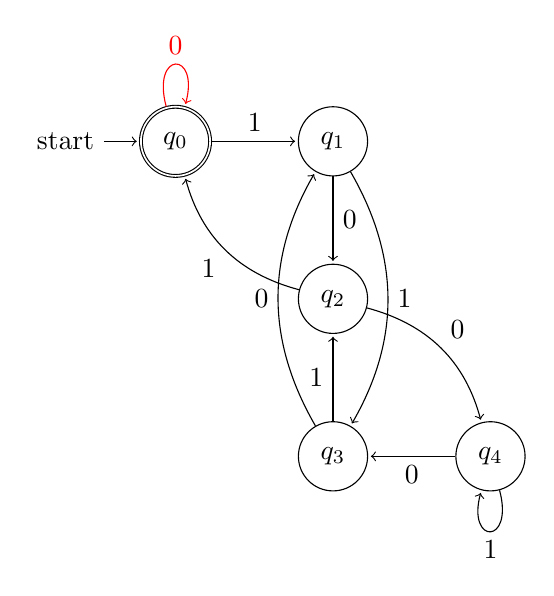
\begin{tikzpicture}[shorten >=1pt,node distance=2cm,on grid,auto]
        \node[state, accepting, initial] (q_0) {$q_0$};
        \node[state] (q_1) [right=of q_0] {$q_1$};
        \node[state] (q_2) [below=of q_1] {$q_2$};
        \node[state] (q_3) [below=of q_2] {$q_3$};
        \node[state] (q_4) [right=of q_3] {$q_4$};
        \path[->]
        (q_0)
        edge [loop above] [color=red] node {0} (q_0)
        edge node {1} (q_1)
        (q_1)
        edge node {0} (q_2)
        edge [bend right=-30] node {1} (q_3)
        (q_2)
        edge [bend left] node {1} (q_0)
        edge [bend right=-30] node {0} (q_4)
        (q_3)
        edge node {1} (q_2)
        edge [bend left] node {0} (q_1)
        (q_4)
        edge node {0} (q_3)
        edge [loop below] node {1} (q_4);
    \end{tikzpicture}
    \caption{DFA, \(A\), this is really beautiful, ya know?}
    \label{fig:multiple5}
\end{figure}


